\documentclass[preview]{standalone}

\usepackage{amsmath}
\usepackage{amssymb}
\usepackage{stellar}
\usepackage{definitions}
\usepackage{tikz}

% https://tex.stackexchange.com/questions/120029/how-to-typeset-a-primed-vector
\newcommand{\pvec}[1]{\vec{#1}\mkern2mu\vphantom{#1}}

\begin{document}

\title{Stellar}
\id{accelerated-reference-frame}
\genpage

\section{Definition}

\begin{snippetdefinition}{accelerated-reference-frame-definition}{Accelerated Reference Frame}
    An \emph{accelerated reference frame} or \emph{non-inertial reference frame}
    is a frame of reference that undergoes acceleration with respect to an inertial frame.
\end{snippetdefinition}

\section{Relativity}

\plain{We want to study the relation between the observations of two distinct observers.}

\begin{snippet}{relative-observers-illustration}
    \begin{center}
        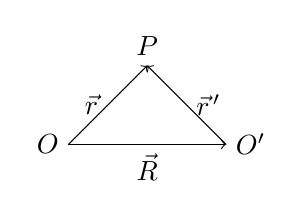
\begin{tikzpicture}[line cap=round,line join=round,scale=1]
            \coordinate (P) at (0, 1);
            \coordinate (O) at (-1, 0);
            \coordinate (Op) at (1, 0);
    
            \node[anchor=east] at (O) {\(O\)};
            \node[anchor=west] at (Op) {\(O'\)};
            \node[anchor=south] at (P) {\(P\)};
    
            \draw[->] (O) -- node[anchor=east] {\(\vec r\)} (P);
            \draw[->] (Op) -- node[anchor=west] {\(\pvec{r}'\)} (P);
            \draw[->] (O) -- node[anchor=north] {\(\vec R\)} (Op);
        \end{tikzpicture}
    \end{center}
\end{snippet}

\begin{snippettheorem}{relation-between-frames-of-reference-theorem}{Relation between frames of reference}
    Consider two observers \(O\) and \(O'\) with coordinate systems \((\hat{x}, \hat{y}, \hat{z})\)
    and \((\hat{u_1}, \hat{u_2}, \hat{u_3})\) respectively.
    Let \(\vec{r}(t)\) be the observation of \(O\) and \(\pvec{r}'(t)\) be the observation of \(O'\)
    of the same particle. Let also \(\vec{R}(t) = \vec{r}(t) - \pvec{r}'(t)\).
    Then,
    \[
        \vec{v}(t) =  \vec{V} + \pvec{v}'(t) + \vec{\omega} \wedge \pvec{r}'(t)
    \]
    and
    \[
        \vec{a} = \vec{A} + \pvec{a}' + 2 \vec{\omega} \wedge \pvec{v}' + \frac{d\vec{\omega}}{dt} \wedge \pvec{r}'
        + \vec{\omega} \wedge (\vec{\omega} \wedge \pvec{r}')
    \]
    The term \(\vec{\omega} \wedge (\vec{\omega} \wedge \pvec{r}')\) is called \emph{centrifugal acceleration},
    the term \(\frac{d\vec{\omega}}{dt} \wedge \pvec{r}'\) is called \emph{Euler acceleration},
    and the term \(2 \vec{\omega} \wedge \pvec{v}'\) is called \emph{Coriolis acceleration}.
\end{snippettheorem}

\begin{snippettheorem}{precession-vector-existence-theorem}{Precession vector}
    There exist a vector \(\vec{\omega}(t)\) such that
    \[
        \frac{d\vec{u_i}}{dt} = \vec{w}(t) \wedge \vec{u_i}
    \]
    with form
    \[
        \vec{\omega}(t) = \frac{1}{2} \sum_{j=1}^3 \hat{u_j} \wedge \frac{d \hat{u_j}}{dt}
    \]
\end{snippettheorem}

\plain{This means that the axis are precessing around the given (non-constant) vector.}

\begin{snippetproof}{relation-between-frames-of-reference-theorem-proof}{relation-between-frames-of-reference-theorem}{Relation between frames of reference}
    The coordinates system are time-dependant for the observer who does not use them, unless both observers coincide.
    We start from
    \[
        \pvec{r}'(t) = \sum_{i=1}^3 x_i'(t)\hat{u_i}(t)
    \]
    By the definition of \(\vec{R}(t)\),
    \[
        \frac{\vec{r}(t)}{dt} = \vec{V}(t) + \frac{d\pvec{r}'}{dt}, \quad \vec{V}(t) = \frac{d\vec{R}(t)}{dt}
    \]
    We now take the derivative to study the last term
    \begin{align*}
        \frac{d\pvec{r}'(t)}{dt} &= \sum_{i=1}^3 \frac{dx_i'(t)}{dt} \hat{u_i}(t)
        + \frac{d\hat{u_i}(t)}{dt} x_i'(t) \\
        &= \sum_{i=1}^3 \frac{dx_i'(t)}{dt} \hat{u_i}(t)
        + \sum_{i=1}^3 \frac{d\hat{u_i}(t)}{dt} x_i'(t) \\
        &= \pvec{v}'(t) + \sum_{i=1}^3 \frac{d\hat{u_i}(t)}{dt} x_i'(t)
    \end{align*}
    Thus,
    \[
        \vec{v} = \vec{V} + \pvec{v}'(t) + \sum_{i=1}^3 \frac{d\hat{u_i}(t)}{dt} x_i'(t)
    \]
    We substitute in the form of the precession motion
    \begin{align*}
        \vec{v} &= \vec{V} + \pvec{v}'(t) + \sum_{i=1}^3 x_i'(\vec{\omega} \wedge \hat{u_i}) \\
        &= \vec{V} + \pvec{v}'(t) + \vec{\omega} \wedge \sum_{i=1}^3 x_i'\hat{u_i} \\
        &= \vec{V} + \pvec{v}'(t) + \vec{\omega} \wedge \pvec{r}'(t)
    \end{align*}
    We now want to find the same relation for the acceleration.
    Since
    \begin{align*}
        \frac{d\pvec{v}'}{dt} &= \sum_{i=1}^3 \left[
            \frac{d^2 x_i'}{dt^2} \hat{u_i} + \frac{dx_i'}{dt} \frac{d\hat{u_i}}{dt}
        \right] \\
        &= \pvec{a}' + \sum_{i=1}^3 \frac{dx_i'}{dt} \frac{d\hat{u_i}}{dt} \\
        &= \pvec{a}' + \sum_{i=1}^3 \frac{dx_i'}{dt} (\vec{\omega} \wedge \hat{u_i}) \\
        &= \pvec{a}' + \vec{\omega} \wedge \sum_{i=1}^3 \frac{dx_i'}{dt} \hat{u_i} \\
        &= \pvec{a}' + \vec{\omega} \wedge \pvec{v}'
    \end{align*}
    we can find the acceleration
    \begin{align*}
        \vec{a} &= \vec{A} + \frac{d\pvec{v}'}{dt} + \frac{d\vec{\omega}}{dt} \wedge \pvec{r}'
        + \vec{\omega} \wedge \frac{d\pvec{r}'}{dt} \\
        &= \vec{A} + \pvec{a}' + 2 \vec{\omega} \wedge \pvec{v}' + \frac{d\vec{\omega}}{dt} \wedge \pvec{r}'
        + \vec{\omega} \wedge (\vec{\omega} \wedge \pvec{r}')
    \end{align*}
\end{snippetproof}

\begin{snippetproof}{precession-vector-existence-theorem-proof}{precession-vector-existence-theorem}{Precession vector}
    We verify that the form of \(\vec{\omega}\) satisfies the given condition:
    \begin{align*}
        (\vec{\omega} \wedge \hat{u_i})_x &= \omega_y u_i^z - \omega_z u_i^y \\
        &= \frac{1}{2} \sum_{j=1}^3 \left\{ u_i^z \left[u_j^z \frac{du_j^x}{dt} - u_j^x \frac{du_j^z}{dt}\right]
        - u_i^y \left[u_j^x \frac{du_j^y}{dt} - u_j^y \frac{du_j^x}{dt}\right] \right\} \\
        &= \frac{1}{2} \sum_{j=1}^3 \left\{
            \frac{du_j^x}{dt} \left[
                u_i^z u_j^z + u_i^yu_j^y
            \right]
            - \frac{du_j^y}{dt} u_i^yu_j^x - \frac{du_j^z}{dt} u_i^zu_j^x
        \right\} \\
        &= \frac{1}{2} \sum_{j=1}^3 \left\{
            \frac{du_j^x}{dt} \left[
                \hat{u_i} \cdot \hat{u_j} - u_i^x u_j^x
            \right]
            - \frac{du_j^y}{dt} u_i^yu_j^x - \frac{du_j^z}{dt} u_i^zu_j^x
        \right\} \\
        &= \frac{1}{2} \sum_{j=1}^3 \left\{
            \frac{du_j^x}{dt} \left[
                \kronecker_{i,j} - u_i^x u_j^x
            \right]
            - \frac{du_j^y}{dt} u_i^yu_j^x - \frac{du_j^z}{dt} u_i^zu_j^x
        \right\} \\
        &= \frac{1}{2} \sum_{j=1}^3 \left\{
            \frac{du_j^x}{dt} \kronecker_{i,j} - u_j^x \left[
                u_i^x \frac{du_j^x}{dt} + \frac{du_j^y}{dt} u_i^y + \frac{du_j^z}{dt} u_i^z
            \right]
        \right\} \\
        &= \frac{1}{2} \frac{du_i^x}{dt} - \frac{1}{2} \sum_{j=1}^3
            u_j^x \left[
                u_i^x \frac{du_j^x}{dt} + \frac{du_j^y}{dt} u_i^y + \frac{du_j^z}{dt} u_i^z
            \right] \\
        &= \frac{1}{2} \frac{du_i^x}{dt} - \frac{1}{2} \sum_{j=1}^3
            u_j^x \left[
                \hat{u_i} \cdot \frac{d\hat{u_j}}{dt}
            \right]
    \end{align*}
    Since
    \[
        0 = \frac{\hat{u_i}}{dt} \cdot \hat{u_j} + \hat{u_i} \frac{\hat{u_j}}{dt}
    \]
    we have that
    \[
        \hat{u_i} \frac{\hat{u_j}}{dt} = - \frac{\hat{u_i}}{dt} \cdot \hat{u_j}
    \]
    and thus
    \begin{align*}
        (\vec{\omega} \wedge \hat{u_i})_x &= \omega_y u_i^z - \omega_z u_i^y \\
        &= \frac{1}{2} \frac{du_i^x}{dt} + \frac{1}{2} \sum_{j=1}^3
        u_j^x \left[
            \hat{u_j} \cdot \frac{d\hat{u_i}}{dt}
        \right] \\
        &= \frac{1}{2} \frac{du_i^x}{dt} + \frac{1}{2} \frac{du_i^x}{dt} \\
        &= \frac{du_i^x}{dt}
    \end{align*}
    By repeating this process for every axis, we get
    \[
        (\vec{\omega} \wedge \hat{u_i})_x = \frac{du_i^x}{dt}
        \qquad
        (\vec{\omega} \wedge \hat{u_i})_y = \frac{du_i^y}{dt}
        \qquad
        (\vec{\omega} \wedge \hat{u_i})_z = \frac{du_i^z}{dt}
    \]
\end{snippetproof}

\end{document}